\begin{center}
\begin{tabular}{| c | c | c | c | c | c | c | c | c | c | c | c | c | c |}
\hline
element & H$_2$NNH$_2$ & HNNH & N & N$_2$ & N$_2$H & N$_2$H$_2$ & N$_2$H$_3$ & NH & NH$_2$ & NH$_3$ & formation energy\\
\hline

Cr & 1.28 & 1.21 & -0.44 &  & 0.12 &  & -0.73 & 0.55 & -0.68 & -0.67 & 3.94 \\
Hf & 1.21 & 1.32 & 1.59 & -0.02 & 0.97 & 0.6 & 0.2 & 0.02 & -1.26 & -0.95 & -0.92 \\
Ru & 0.82 & 0.76 & 0.48 & -0.83 & 0.64 & 0.17 & 0.57 & 0.86 & -0.76 & -1.13 & 5.45 \\
Os & 0.61 & 0.39 & -0.7 & -1.17 & -0.15 & -0.36 & 0.06 & 0.06 & -1.26 & -1.29 & 6.31 \\
W & 1.25 & 0.84 & -1.8 & -0.37 & -0.24 & -0.73 & 0.01 & -1.06 & -1.43 & -0.8 & 3.99 \\
Pt &  & 2.16 & 2.77 & 0.26 & 1.78 & 2.06 & 1.44 & 1.69 & 0.08 & -0.09 & 6.86 \\
Y & 1.01 & 1.69 & 2.72 & 0.02 &  & 2.0 & 1.34 & 2.58 & 0.02 & -0.77 & -1.38 \\
Ta & 1.1 & 0.31 & -0.99 & -0.13 & 0.42 & -0.32 & -0.22 & -0.95 & -1.69 & -0.85 & 1.69 \\
Ni & 1.75 & 1.94 & 3.35 & 0.17 & 1.64 & 1.9 & 1.08 &  & 0.12 & -0.43 & 5.58 \\
Sc & 1.06 & 1.76 & 3.51 & 0.03 & 1.7 & 1.59 & 1.0 & 2.18 & -0.43 & -0.76 & -1.71 \\
Zr & 1.23 & 1.39 & 1.71 & -0.01 & 1.07 & 0.74 & 0.35 & 0.16 & -1.09 & -0.88 & -0.51 \\
Re & 0.95 & 0.67 & -1.5 & -0.83 & -0.42 & -0.15 & 0.32 & -0.18 & -1.03 & -0.96 & 5.06 \\
Au & 1.68 & 2.36 & 4.05 & 0.25 & 2.54 &  & 2.15 & 2.95 & 0.92 & -0.08 & 8.18 \\
Ti & 1.42 & 1.64 & 1.73 & 0.11 & 1.27 & 0.85 & 0.61 & 0.37 & -0.82 & -0.6 & 0.0 \\
Mo & 1.27 & 1.11 & -1.2 & -0.33 & 0.01 & 0.09 & 0.51 & -0.24 & -1.03 & -0.75 & 3.26 \\
Tc & 1.03 & 0.95 & -0.87 & -0.65 & 0.06 & 0.27 & 0.65 & 0.52 & -0.69 & -0.92 & 4.58 \\
Ir & 0.82 & 0.74 & 1.03 & -0.7 & 0.26 & 0.19 & -0.01 & 0.54 & -1.34 & -1.2 & 7.07 \\
Cu & 1.33 & 2.07 & 4.51 & 0.18 & 2.33 & 2.4 & 1.65 & 3.41 & 0.95 & -0.45 &  \\
Nb & 1.23 & 0.43 & -1.04 & -0.23 & 0.35 & -0.36 & -0.04 & -0.84 & -1.52 & -0.86 & 1.5 \\
Ag & 1.44 & 2.33 & 5.3 & 0.24 & 2.62 & 2.65 & 2.04 & 3.83 & 1.29 & -0.18 & 7.28 \\
Pd & 1.53 & 2.12 & 3.55 & 0.23 & 2.0 & 2.25 & 1.67 & 2.5 & 0.44 & -0.22 & 6.08 \\
V & 1.43 & 1.5 & -0.33 & 0.04 & 0.82 & 0.38 & 0.55 & 0.17 & -0.86 & -1.03 & 2.48 \\
Co & 1.14 & 1.53 & 2.34 & 0.12 & 1.04 & 1.05 & 0.78 & 1.82 & -0.57 & -0.72 & 4.49 \\
Rh & 1.16 & 1.3 & 1.86 & -0.16 & 0.71 & 0.85 & 0.44 & 1.34 & -0.88 & -0.87 & 6.01 \\
\hline
\end{tabular}
\caption{The calculated relative energies of all surface species on all metal substituents at standard state. All energies are referenced with respect to N$_2$ gas and H$_2$ gas at 300K and 1 bar of pressure. Blank spaces represent calculations that could not be converged}
\label{table:energies}
\end{center}



\begin{figure}
\centering
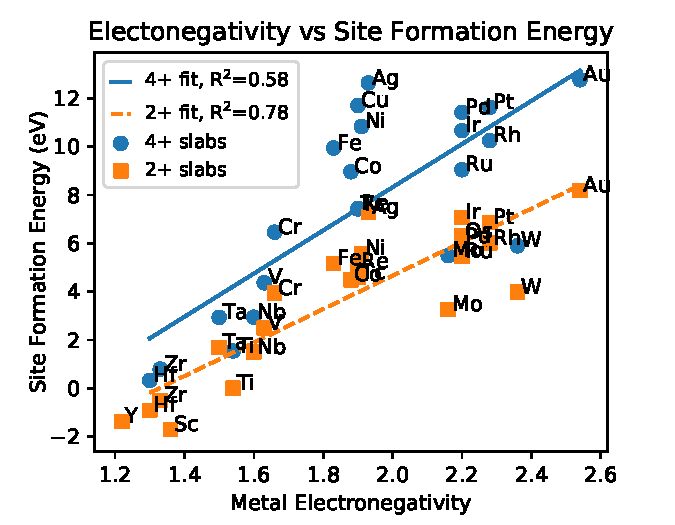
\includegraphics[width=0.8\linewidth]{Images/electronegativity_vs_formation.pdf}
\caption{Electronegativity vs formation energy of 2+ dopant site}
\end{figure}

\begin{figure}
\centering
\includegraphics[width=0.8\linewidth]{data/plotsTi_associative.pdf}
\end{figure}

\begin{figure}
\centering
\includegraphics[width=0.8\linewidth]{data/plotsIr_distal_2.pdf}
\end{figure}

\begin{figure}
\centering
\includegraphics[width=0.8\linewidth]{data/plotsV_associative_2.pdf}
\end{figure}

\begin{figure}
\centering
\includegraphics[width=0.8\linewidth]{data/plotsMo_distal_1.pdf}
\end{figure}

\begin{figure}
\centering
\includegraphics[width=0.8\linewidth]{data/plotsPt_dissociative.pdf}
\end{figure}

\begin{figure}
\centering
\includegraphics[width=0.8\linewidth]{data/plotsNb_distal_1.pdf}
\end{figure}

\begin{figure}
\centering
\includegraphics[width=0.8\linewidth]{data/plotsRu_distal_2.pdf}
\end{figure}

\begin{figure}
\centering
\includegraphics[width=0.8\linewidth]{data/plotsAu_dissociative.pdf}
\end{figure}

\begin{figure}
\centering
\includegraphics[width=0.8\linewidth]{data/plotsCu_dissociative.pdf}
\end{figure}

\begin{figure}
\centering
\includegraphics[width=0.8\linewidth]{data/plotsPd_distal_1.pdf}
\end{figure}

\begin{figure}
\centering
\includegraphics[width=0.8\linewidth]{data/plotsRh_dissociative.pdf}
\end{figure}

\begin{figure}
\centering
\includegraphics[width=0.8\linewidth]{data/plotsIr_dissociative.pdf}
\end{figure}

\begin{figure}
\centering
\includegraphics[width=0.8\linewidth]{data/plotsRh_distal_1.pdf}
\end{figure}

\begin{figure}
\centering
\includegraphics[width=0.8\linewidth]{data/plotsTc_associative_2.pdf}
\end{figure}

\begin{figure}
\centering
\includegraphics[width=0.8\linewidth]{data/plotsRu_associative_2.pdf}
\end{figure}

\begin{figure}
\centering
\includegraphics[width=0.8\linewidth]{data/plotsW_distal_1.pdf}
\end{figure}

\begin{figure}
\centering
\includegraphics[width=0.8\linewidth]{data/plotsSc_associative_2.pdf}
\end{figure}

\begin{figure}
\centering
\includegraphics[width=0.8\linewidth]{data/plotsOs_distal_2.pdf}
\end{figure}

\begin{figure}
\centering
\includegraphics[width=0.8\linewidth]{data/plotsV_dissociative.pdf}
\end{figure}

\begin{figure}
\centering
\includegraphics[width=0.8\linewidth]{data/plotsSc_dissociative.pdf}
\end{figure}

\begin{figure}
\centering
\includegraphics[width=0.8\linewidth]{data/plotsRe_associative.pdf}
\end{figure}

\begin{figure}
\centering
\includegraphics[width=0.8\linewidth]{data/plotsAg_distal_2.pdf}
\end{figure}

\begin{figure}
\centering
\includegraphics[width=0.8\linewidth]{data/plotsCu_associative_2.pdf}
\end{figure}

\begin{figure}
\centering
\includegraphics[width=0.8\linewidth]{data/plotsRh_distal_2.pdf}
\end{figure}

\begin{figure}
\centering
\includegraphics[width=0.8\linewidth]{data/plotsIr_distal_1.pdf}
\end{figure}

\begin{figure}
\centering
\includegraphics[width=0.8\linewidth]{data/plotsCu_distal_2.pdf}
\end{figure}

\begin{figure}
\centering
\includegraphics[width=0.8\linewidth]{data/plotsPt_distal_2.pdf}
\end{figure}

\begin{figure}
\centering
\includegraphics[width=0.8\linewidth]{data/plotsRh_associative.pdf}
\end{figure}

\begin{figure}
\centering
\includegraphics[width=0.8\linewidth]{data/plotsOs_dissociative.pdf}
\end{figure}

\begin{figure}
\centering
\includegraphics[width=0.8\linewidth]{data/plotsRh_associative_2.pdf}
\end{figure}

\begin{figure}
\centering
\includegraphics[width=0.8\linewidth]{data/plotsV_distal_2.pdf}
\end{figure}

\begin{figure}
\centering
\includegraphics[width=0.8\linewidth]{data/plotsTa_distal_2.pdf}
\end{figure}

\begin{figure}
\centering
\includegraphics[width=0.8\linewidth]{data/plotsCo_distal_1.pdf}
\end{figure}

\begin{figure}
\centering
\includegraphics[width=0.8\linewidth]{data/plotsRu_dissociative.pdf}
\end{figure}

\begin{figure}
\centering
\includegraphics[width=0.8\linewidth]{data/plotsW_dissociative.pdf}
\end{figure}

\begin{figure}
\centering
\includegraphics[width=0.8\linewidth]{data/plotsTc_dissociative.pdf}
\end{figure}

\begin{figure}
\centering
\includegraphics[width=0.8\linewidth]{data/plotsTc_associative.pdf}
\end{figure}

\begin{figure}
\centering
\includegraphics[width=0.8\linewidth]{data/plotsHf_associative.pdf}
\end{figure}

\begin{figure}
\centering
\includegraphics[width=0.8\linewidth]{data/plotsOs_associative_2.pdf}
\end{figure}

\begin{figure}
\centering
\includegraphics[width=0.8\linewidth]{data/plotsIr_associative.pdf}
\end{figure}

\begin{figure}
\centering
\includegraphics[width=0.8\linewidth]{data/plotsCu_distal_1.pdf}
\end{figure}

\begin{figure}
\centering
\includegraphics[width=0.8\linewidth]{data/plotsRe_dissociative.pdf}
\end{figure}

\begin{figure}
\centering
\includegraphics[width=0.8\linewidth]{data/plotsTa_associative_2.pdf}
\end{figure}

\begin{figure}
\centering
\includegraphics[width=0.8\linewidth]{data/plotsCo_associative_2.pdf}
\end{figure}

\begin{figure}
\centering
\includegraphics[width=0.8\linewidth]{data/plotsMo_associative_2.pdf}
\end{figure}

\begin{figure}
\centering
\includegraphics[width=0.8\linewidth]{data/plotsNb_associative.pdf}
\end{figure}

\begin{figure}
\centering
\includegraphics[width=0.8\linewidth]{data/plotsPd_associative.pdf}
\end{figure}

\begin{figure}
\centering
\includegraphics[width=0.8\linewidth]{data/plotsTc_distal_2.pdf}
\end{figure}

\begin{figure}
\centering
\includegraphics[width=0.8\linewidth]{data/plotsCo_dissociative.pdf}
\end{figure}

\begin{figure}
\centering
\includegraphics[width=0.8\linewidth]{data/plotsMo_associative.pdf}
\end{figure}

\begin{figure}
\centering
\includegraphics[width=0.8\linewidth]{data/plotsPd_distal_2.pdf}
\end{figure}

\begin{figure}
\centering
\includegraphics[width=0.8\linewidth]{data/plotsNb_associative_2.pdf}
\end{figure}

\begin{figure}
\centering
\includegraphics[width=0.8\linewidth]{data/plotsW_associative.pdf}
\end{figure}

\begin{figure}
\centering
\includegraphics[width=0.8\linewidth]{data/plotsAg_dissociative.pdf}
\end{figure}

\begin{figure}
\centering
\includegraphics[width=0.8\linewidth]{data/plotsY_dissociative.pdf}
\end{figure}

\begin{figure}
\centering
\includegraphics[width=0.8\linewidth]{data/plotsNb_dissociative.pdf}
\end{figure}

\begin{figure}
\centering
\includegraphics[width=0.8\linewidth]{data/plotsSc_distal_1.pdf}
\end{figure}

\begin{figure}
\centering
\includegraphics[width=0.8\linewidth]{data/plotsNb_distal_2.pdf}
\end{figure}

\begin{figure}
\centering
\includegraphics[width=0.8\linewidth]{data/plotsW_distal_2.pdf}
\end{figure}

\begin{figure}
\centering
\includegraphics[width=0.8\linewidth]{data/plotsTa_dissociative.pdf}
\end{figure}

\begin{figure}
\centering
\includegraphics[width=0.8\linewidth]{data/plotsTc_distal_1.pdf}
\end{figure}

\begin{figure}
\centering
\includegraphics[width=0.8\linewidth]{data/plotsRe_distal_1.pdf}
\end{figure}

\begin{figure}
\centering
\includegraphics[width=0.8\linewidth]{data/plotsTi_associative_2.pdf}
\end{figure}

\begin{figure}
\centering
\includegraphics[width=0.8\linewidth]{data/plotsRu_distal_1.pdf}
\end{figure}

\begin{figure}
\centering
\includegraphics[width=0.8\linewidth]{data/plotsV_associative.pdf}
\end{figure}

\begin{figure}
\centering
\includegraphics[width=0.8\linewidth]{data/plotsNi_associative.pdf}
\end{figure}

\begin{figure}
\centering
\includegraphics[width=0.8\linewidth]{data/plotsHf_associative_2.pdf}
\end{figure}

\begin{figure}
\centering
\includegraphics[width=0.8\linewidth]{data/plotsRe_associative_2.pdf}
\end{figure}

\begin{figure}
\centering
\includegraphics[width=0.8\linewidth]{data/plotsIr_associative_2.pdf}
\end{figure}

\begin{figure}
\centering
\includegraphics[width=0.8\linewidth]{data/plotsAg_associative_2.pdf}
\end{figure}

\begin{figure}
\centering
\includegraphics[width=0.8\linewidth]{data/plotsHf_distal_2.pdf}
\end{figure}

\begin{figure}
\centering
\includegraphics[width=0.8\linewidth]{data/plotsRe_distal_2.pdf}
\end{figure}

\begin{figure}
\centering
\includegraphics[width=0.8\linewidth]{data/plotsSc_associative.pdf}
\end{figure}

\begin{figure}
\centering
\includegraphics[width=0.8\linewidth]{data/plotsTi_distal_2.pdf}
\end{figure}

\begin{figure}
\centering
\includegraphics[width=0.8\linewidth]{data/plotsMo_dissociative.pdf}
\end{figure}

\begin{figure}
\centering
\includegraphics[width=0.8\linewidth]{data/plotsZr_dissociative.pdf}
\end{figure}

\begin{figure}
\centering
\includegraphics[width=0.8\linewidth]{data/plotsRu_associative.pdf}
\end{figure}

\begin{figure}
\centering
\includegraphics[width=0.8\linewidth]{data/plotsAg_distal_1.pdf}
\end{figure}

\begin{figure}
\centering
\includegraphics[width=0.8\linewidth]{data/plotsOs_associative.pdf}
\end{figure}

\begin{figure}
\centering
\includegraphics[width=0.8\linewidth]{data/plotsAg_associative.pdf}
\end{figure}

\begin{figure}
\centering
\includegraphics[width=0.8\linewidth]{data/plotsCo_distal_2.pdf}
\end{figure}

\begin{figure}
\centering
\includegraphics[width=0.8\linewidth]{data/plotsTa_distal_1.pdf}
\end{figure}

\begin{figure}
\centering
\includegraphics[width=0.8\linewidth]{data/plotsZr_distal_2.pdf}
\end{figure}

\begin{figure}
\centering
\includegraphics[width=0.8\linewidth]{data/plotsTa_associative.pdf}
\end{figure}

\begin{figure}
\centering
\includegraphics[width=0.8\linewidth]{data/plotsPt_distal_1.pdf}
\end{figure}

\begin{figure}
\centering
\includegraphics[width=0.8\linewidth]{data/plotsCu_associative.pdf}
\end{figure}

\begin{figure}
\centering
\includegraphics[width=0.8\linewidth]{data/plotsPd_associative_2.pdf}
\end{figure}

\begin{figure}
\centering
\includegraphics[width=0.8\linewidth]{data/plotsPd_dissociative.pdf}
\end{figure}

\begin{figure}
\centering
\includegraphics[width=0.8\linewidth]{data/plotsCo_associative.pdf}
\end{figure}

\begin{figure}
\centering
\includegraphics[width=0.8\linewidth]{data/plotsV_distal_1.pdf}
\end{figure}

\begin{figure}
\centering
\includegraphics[width=0.8\linewidth]{data/plotsTi_dissociative.pdf}
\end{figure}

\begin{figure}
\centering
\includegraphics[width=0.8\linewidth]{data/plotsMo_distal_2.pdf}
\end{figure}

\begin{figure}
\centering
\includegraphics[width=0.8\linewidth]{data/plotsSc_distal_2.pdf}
\end{figure}

\begin{figure}
\centering
\includegraphics[width=0.8\linewidth]{data/plotsZr_associative_2.pdf}
\end{figure}

\begin{figure}
\centering
\includegraphics[width=0.8\linewidth]{data/plotsZr_associative.pdf}
\end{figure}

\begin{figure}
\centering
\includegraphics[width=0.8\linewidth]{data/plotsOs_distal_1.pdf}
\end{figure}

\begin{figure}
\centering
\includegraphics[width=0.8\linewidth]{data/plotsTi_distal_1.pdf}
\end{figure}

\begin{figure}
\centering
\includegraphics[width=0.8\linewidth]{data/plotsHf_dissociative.pdf}
\end{figure}

\begin{figure}
\centering
\includegraphics[width=0.8\linewidth]{data/plotsW_associative_2.pdf}
\end{figure}

\begin{figure}
\centering
\includegraphics[width=0.8\linewidth]{data/plotsZr_distal_1.pdf}
\end{figure}

\begin{figure}
\centering
\includegraphics[width=0.8\linewidth]{data/plotsHf_distal_1.pdf}
\end{figure}

